 \thispagestyle{gocconone}
\pagestyle{gocco}
\everymath{\color{gocco}}
\graphicspath{{../gocco/pic/}}
\blfootnote{$^1${\color[named]{gocco}Trung tâm Ứng dụng Công nghệ Vũ trụ Tp. Hồ Chí Minh.}}
\begingroup
\AddToShipoutPicture*{\put(0,616){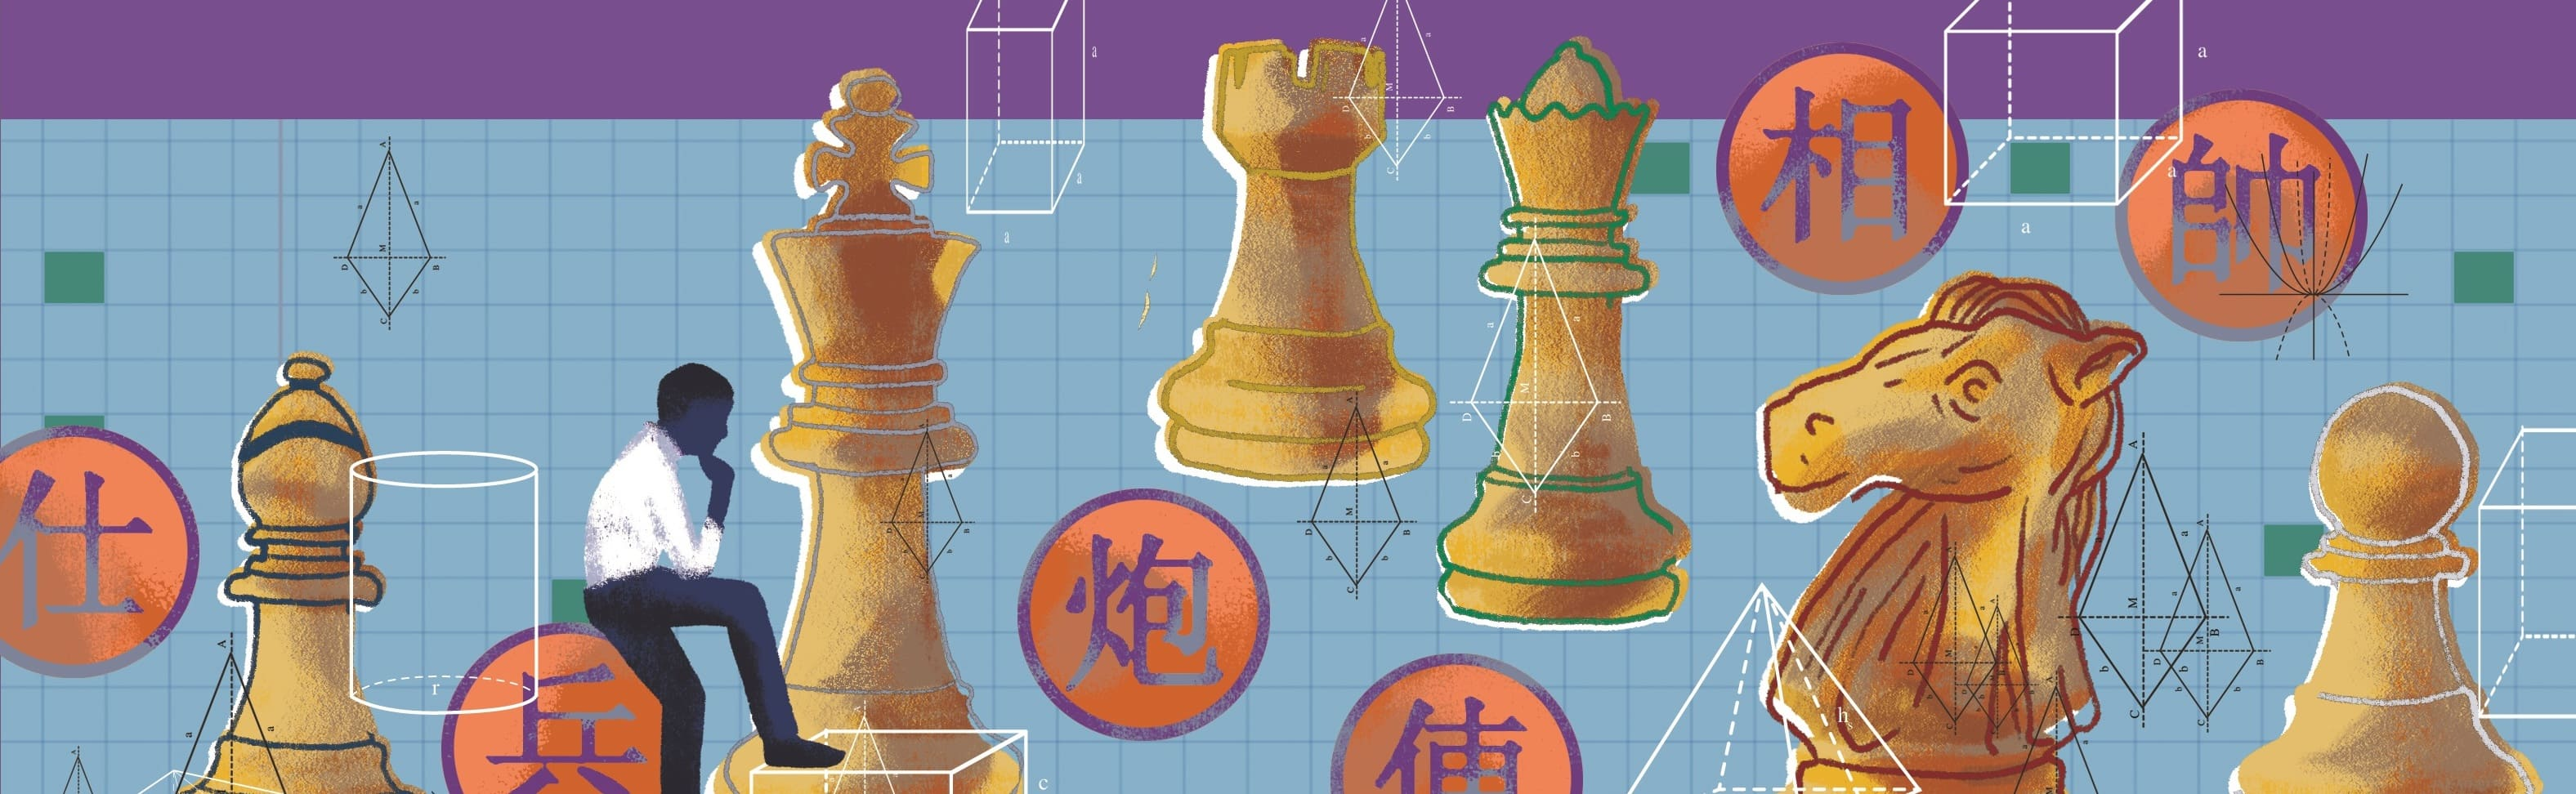
\includegraphics[width=19.3cm]{../bannergocco}}}
\AddToShipoutPicture*{\put(128,550){
\includegraphics[scale=1]{../tieude2.pdf}}} 
\centering
\endgroup

\vspace*{155pt}
\begin{multicols}{2}	
	Trong những diễn biến phức tạp của ván đấu, việc một bên chủ động bỏ một hoặc nhiều quân chủ lực để đạt được những mục đích khác nhau như: tranh tiên, đoạt thế, công sát, giải vây \ldots từ đó giành lấy kết quả có lợi sau cùng, được gọi là \textit{Chiến thuật thí quân}. Thí quân có thể diễn ra bất cứ giai đoạn nào, nhưng phổ biến nhất là ở giai đoạn Trung Cuộc. Một khi chiến thuật này được vận dụng, ván đấu sẽ phát sinh những tình huống khó lường, tạo ra những bất ngờ cho đối thủ cũng như xoay chuyển kết quả thắng -- thua của toàn bộ cuộc chiến.
	\vskip 0.1cm
	\textit{Chiến thuật thí quân} cũng phản ánh một cách rõ mối liên hệ giữa $2$ yếu tố \textit{Quân} và \textit{Thế}: Bên thí quân chịu thiệt thòi là bị mất đi quân chiến nhưng bù lại sẽ có được một hình thế có lợi hơn. Do vậy trước khi tiến hành vận dụng chiến thuật này trong thực chiến, đòi hỏi người cầm quân phải có sự tính toán cực kỳ tỉ mỉ và chuẩn xác về những nước đi cũng như những tình huống sẽ diễn ra tiếp theo, từ đó việc thực hiện có thể được diễn ra liền mạch để có thể đạt được mục tiêu đề~ra.
	\vskip 0.1cm
	Để cảm nhận rõ hơn về chiến thuật thú vị này, tác giả sẽ gửi tới bạn đọc của Pi vài ví dụ  để có thể  áp dụng trong những ván đấu thực chiến:
	\vskip 0.1cm
	$1.$ Hình $1$, thoạt nhìn có vẻ như bên Đen đang nắm lợi thế lớn với $3$ quân tấn công đang áp sát Tướng Đỏ và chỉ cần đi X$6.2$ là tạo sát ngay lập tức. Bên Đỏ mặc dù chưa có thế tấn công rõ ràng, nhưng với lợi thế đi tiên, Đỏ đã áp dụng chiến thuật thí quân để xoay chuyển cục diện như sau:
	\begin{figure}[H]
		\vspace*{-5pt}
		\centering
		\captionsetup{labelformat= empty, justification=centering}
		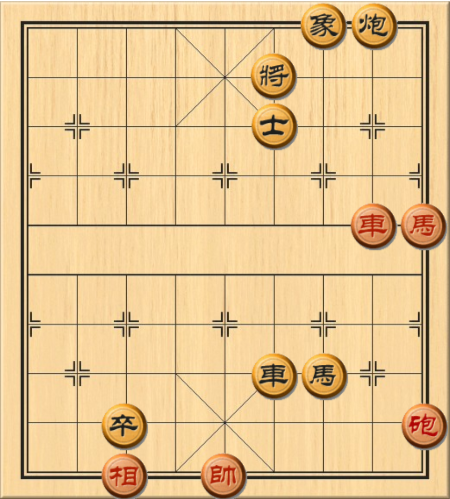
\includegraphics[width= 0.4\textwidth]{1}
		\caption{\small\textit{\color{gocco}Hình $1$.}}
		\vspace*{-10pt}
	\end{figure}
	$\pmb{1)}$ X$2.3$ Tg$6/1$\quad  $\pmb{2)}$ X$2-4$ Tg$6.1$\quad $\pmb{3)}$ M$1.3$ Tg$6/1$ ($*$)\quad $\pmb{4)}$ M$3.2$ Tg$6.1$\quad  $\pmb{5)}$ P$1.7$ ($**$) ($1-0$)
	\vskip 0.1cm
	\textit{($*$): Với việc có mặt Tướng hỗ trợ ở Trung lộ  Đỏ liên tục tấn Xe rồi Phế Xe ép Đen phải đưa ra lựa chọn duy nhất là dùng Tướng ăn Xe đối phương. 
	\vskip 0.1cm
	($**$): Sau khi dùng đòn hi sinh, Đỏ tiếp tục điều Mã tới vị trí thuận lợi, tạo điều kiện cho Pháo tấn lên tạo đòn sát cục Tiền Mã Hậu Pháo kinh điển, Đen không thể làm gì hơn, đành chấp nhận thất bại.}
	\begin{figure}[H]
		\vspace*{-5pt}
		\centering
		\captionsetup{labelformat= empty, justification=centering}
		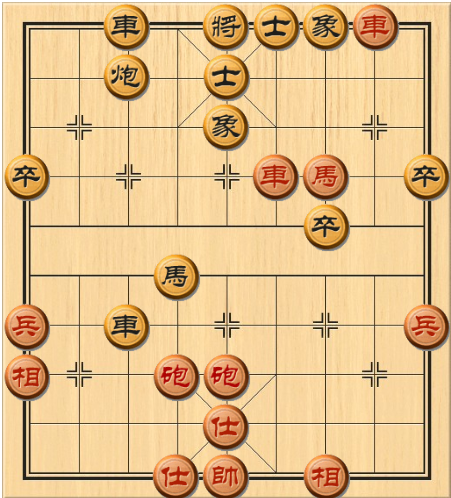
\includegraphics[width= 0.4\textwidth]{2}
		\caption{\small\textit{\color{gocco}Hình $2$.}}
		\vspace*{-10pt}
	\end{figure}
	$2.$ Hình $2$, tình huống cờ Trung cuộc đang khá phức tạp. Mặc dù Đen kém quân nhưng có vẻ vẫn còn có thể chống đỡ lâu dài. Tuy nhiên,  Đỏ đi trước và đã nhìn ra được điểm yếu cánh trái không có quân phòng thủ của Đen, ngay lập tức Đỏ tung ra đòn thí quân tạo thế sát như sau:
	\vskip 0.1cm
	$\pmb{1)}$ X$4.3$ ($*$) Tg$5-6$\quad $\pmb{2)}$ M$3.5$ P$3.1$\quad  $\pmb{3)}$ M$5/3$ P$3-7$\quad $\pmb{4)}$ X$2-3$  Tg$6.1$\quad $\pmb{5)}$ X$3/2$ ($**$) ($1-0$)
	\vskip 0.1cm
	\textit{($*$): Một nước đi bất ngờ và đầy quyết đoán của Đỏ, buộc Tướng Đen phải ăn ra, mở đường cho quân Mã nhảy lên chém Tượng ở lộ $5$ ở nước kế tiếp;
	\vskip 0.1cm
	($**$): Mặc dù đã nhìn thấy trước nhưng Đen không cũng có cách nào chống lại nước X$3.2$ sát cục của Đỏ. Đen thua cuộc.}
	\vskip 0.1cm
	$3.$ Hình $3$, Xe Đen đang bắt Mã Đỏ nhưng lại có cánh trái khá trống trải. Được quyền đi trước, Đỏ biết thời cơ đã tới, không chạy Mã mà có những nước tấn công đầy dứt khoát như sau:
	\vskip 0.1cm
	$\pmb{1)}$	X$3.4$ X$3.2$ ($*$)\quad  $\pmb{2)}$ M$6.4$ P$9-6$\quad  $\pmb{3)}$ X$3.4$ S$5/6$\quad $\pmb{4)}$ P$t.4$ ($**$) X$3.1$\quad $\pmb{5)}$ S$4.5$ X$3/4$ \quad $\pmb{6)}$ Pt$-7$ X$3-2$\quad $\pmb{7)}$ P$6.6$ ($***$) X$2/4$\quad $\pmb{8)}$ P$6/3$ X$2-3$\quad $\pmb{9)}$ P$7-6$ M$4.3$\quad $\pmb{10)}$ X$3/2$ P$6/1$\quad $\pmb{11)}$ Ps$-2$ P$6-8$\quad $\pmb{12)}$ X$3-5$ ($1-0$)
	\vskip 0.1cm
	\textit{($*$): Lúc này nếu Đen không ăn lại Mã Đỏ cũng khó tìm ra giải pháp nào tốt hơn. Nếu thay vào đỏ, Đen đi T$7.5$, diễn biến tiếp theo có thể như sau: $\pmb{2)}$ M$6.5$ P$9-6$\quad $\pmb{3)}$ Pt$.4$ P$6-4$\quad $\pmb{4)}$ X$3.4$ S$5/6$\quad $\pmb{5)}$ M$5.3$ Tg$5.1$\quad $\pmb{6)}$ P$6.5$ (Đỏ có thế công mạnh mẽ, nắm chắc phần thắng)
	\vskip 0.1cm
	($**$): Đỏ tiếp tục tăng cường sức ép lên trận hình đối thủ, trước nhảy Mã tới dọa chiếu ở vị trí ngọa tào, sau đánh Tượng chiếu rồi ăn lại Pháo, chính thức xác lập ưu thế tuyệt đối.
	\vskip 0.1cm
	($***$): Đỏ tiếp tục đoạt thêm $1$ Mã của Đen, chiến thắng dành cho Đỏ chỉ còn là vấn đề thời gian.
	\vskip 0.1cm
	($****$): Lúc này Đen có chống Sỹ bên nào cũng đều bị Đỏ nhảy M$3.4$ và phối hợp Xe và $2$ Pháo chiếu bí. Đen đành chấp nhận thất bại.}
	\begin{figure}[H]
		\vspace*{-5pt}
		\centering
		\captionsetup{labelformat= empty, justification=centering}
		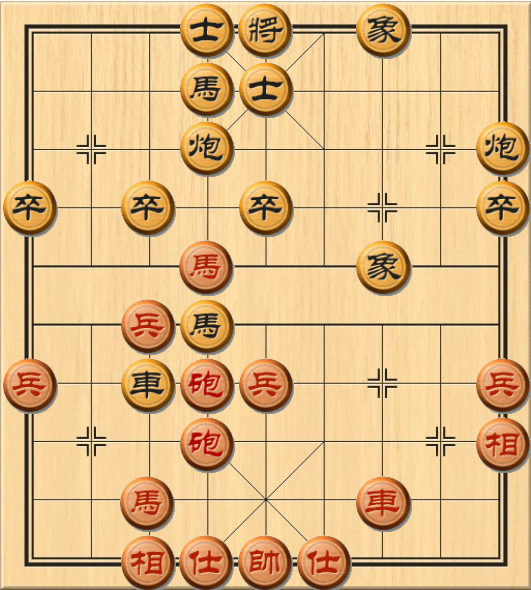
\includegraphics[width= 0.4\textwidth]{3}
		\caption{\small\textit{\color{gocco}Hình $3$}}
		\vspace*{-10pt}
	\end{figure}
	\textit{Chú thích:} C: Chốt, X: Xe, M: Mã, P: Pháo, Tg: Tướng, S: Sĩ, T: Tượng, t: trước, s: Sau. 
	\vskip 0.1cm
	\textbf{\color{gocco}Câu đố kỳ này:} Đỏ được quyền đi trước, sẽ áp dụng chiến thuật thí quân như thế nào để giành lấy thắng lợi trong những hình cờ dưới đây?
	\begin{figure}[H]
		\vspace*{5pt}
		\centering
		\captionsetup{labelformat= empty, justification=centering}
		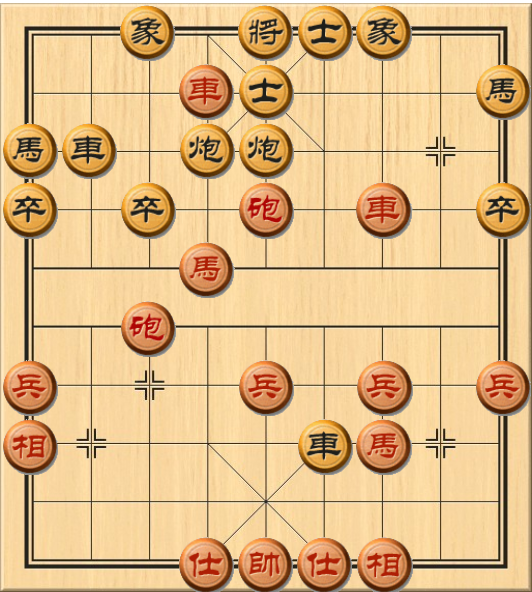
\includegraphics[width= 0.4\textwidth]{4}
		\caption{\small\textit{\color{gocco}Hình $4$.}}
		\vspace*{-10pt}
	\end{figure}
	\begin{figure}[H]
		\vspace*{5pt}
		\centering
		\captionsetup{labelformat= empty, justification=centering}
		
\includegraphics[width= 0.4\textwidth]{5}
		\caption{\small\textit{\color{gocco}Hình $5$.}}
		\vspace*{-10pt}
	\end{figure}
\end{multicols}
\vspace*{-10pt}
{\color{gocco}\rule{1\linewidth}{0.1pt}}

\vspace*{10pt}
\centerline{\LARGE\textbf{\color{gocco}LỜI GIÁI, ĐÁP ÁN}} 
\begin{multicols}{2}
	\textbf{\color{gocco}Đố vui}
	\vskip 0.1cm
	Khi mỗi khối gỗ tròn lăn về phía trước, điểm tiếp xúc với khối gỗ bên trên di chuyển về phía sau; vì vậy khi khối gỗ tròn lăn được một vòng thì khối gỗ bên trên di chuyển được về phía trước $1$m so với khối gỗ tròn. Tuy nhiên, khối gỗ tròn cũng di chuyển được $1$m về phía trước so với mặt đất. Vì thế khối gỗ bên trên di chuyển được một khoảng cách là $2$m so với mặt đất. 
	\vskip 0.1cm
	\textbf{\color{gocco}Hai băng cướp bị tóm gọn}
	\vskip 0.1cm
	Đối với mỗi tên thuộc băng Mèo rừng ta sẽ đánh dấu bằng màu đỏ tên cướp thuộc băng Báo đen nào to béo nhất ngồi cạnh hắn ta (nếu hai tên Báo đen nặng như nhau ngồi cạnh, ta sẽ chọn lấy đúng một tên bất kỳ; hoặc nếu chỉ có một tên Báo đen ngồi cạnh thì ta sẽ chọn đúng tên đó). Như vậy mỗi tên cướp ở băng Báo đen được đánh dấu sẽ ngồi cạnh một tên thuộc băng Mèo rừng gầy còm hơn hắn ta.
	\vskip 0.1cm
	Giả sử không phải tất cả các tên thuộc băng Báo đen được đánh dấu đỏ. Khi đó số các tên thuộc băng Báo đen được đánh dấu sẽ nhỏ hơn hoặc bằng $9$. Vì mỗi tên thuộc băng Báo đen chỉ có thể ngồi cạnh không quá $2$ tên thuộc băng Mèo rừng, suy ra bên cạnh các tên cướp được đánh dấu đỏ thuộc băng Báo đen có không quá $18$ tên thuộc băng Mèo rừng, số lượng này ít hơn tổng số các tên cướp thuộc băng Mèo rừng là $19$ tên. Ta nhận được mâu thuẫn, do tất cả các tên cướp thuộc băng Mèo rừng đều phải ngổi cạnh một tên thuộc băng Báo đen được đánh dấu đỏ.
	\vskip 0.1cm
	Như vậy, mỗi tên thuộc băng Báo đen phải có một tên thuộc băng Mèo rừng gầy còm hơn ngồi cạnh.
	\vskip 0.1cm
	\textbf{\color{gocco}Góc cờ}
	\vskip 0.1cm
	Hình $4$: 
	\vskip 0.1cm
	$\pmb{1)}$ X$3.3$ M$9/7$\quad $\pmb{2)}$ M$6.5$ X$6/5$\quad $\pmb{3)}$ P$7-6$ P$4.7$\quad $\pmb{4)}$ X$6.1$  Tg$5-4$\quad  $\pmb{5)}$ P$5-6$ Tg$4-5$\quad $\pmb{6)}$ M$5.7$ ($1-0$)
	\vskip 0.1cm
	Hình $5$: $\pmb{1)}$ P$5.2$ S$6.5$\quad $\pmb{2)}$ X$4.6$ X$8/6$\quad  $\pmb{3)}$ X$4-5$ P$4-3$\quad $\pmb{4)}$ X$3-8$  M$9.7$\quad  $\pmb{5)}$ X$5-7$ Tg$4-5$\quad $\pmb{6)}$ M$7.6$ P$3-2$\quad $\pmb{7)}$ X$8.3$ X$4/3$\quad $\pmb{8)}$ X$7-3$ M$7/9$\quad $\pmb{9)}$ X$3-9$ M$9.7$\quad $\pmb{10)}$ X$8/1$ M$7.5$\quad  $\pmb{11)}$ X$8.2$ T$5/3$\quad $\pmb{12)}$ X$8-5$ Tg$5-4$\quad $\pmb{13)}$ X$9-7$ T$3.1$\quad $\pmb{14)}$ X$7-8$  ($1-0$)
\end{multicols}



